  \documentclass[supercite]{Experimental_Report}



\title{~~~~~~数据结构实验~~~~~~}
\author{周泽栩}
%\coauthor{张三、李四}
\school{计算机科学与技术学院}
\classnum{CS启明2401}
\stunum{U202414896}
%\costunum{U202115631、U202115631}
\instructor{蔡宇杰} % 该系列实验报告模板有华科大计院教师陈加忠制作
\date{2026年1月5日}

\usepackage{listings} % 引入代码高亮宏包
\usepackage{xcolor}   % 用于代码高亮的颜色

% 配置代码高亮的样式
\lstset{
    basicstyle=\ttfamily\small, % 设置代码字体和大小
    commentstyle=\color{gray}, % 注释颜色
    keywordstyle=\color{blue}, % 关键字颜色
    stringstyle=\color{red},   % 字符串颜色
    breaklines=true,           % 自动换行
    numbers=left,              % 行号在左侧显示
    numberstyle=\tiny\color{gray}, % 行号样式
    frame=shadowbox,           % 代码框阴影
    rulesepcolor=\color{gray}  % 框线颜色
}

\usepackage{algorithm, multirow}
\usepackage{algpseudocode}
\usepackage{amsmath}
\usepackage{amsthm}
\usepackage{framed}
\usepackage{mathtools}
\usepackage{subcaption}
\usepackage{xltxtra} %提供了针对XeTeX的改进并且加入了XeTeX的LOGO, 自动调用xunicode宏包(提供Unicode字符宏)
\usepackage{bm}
\usepackage{tikz}
\usepackage{tikzscale}
\usepackage{pgfplots}
%\usepackage{enumerate}

\pgfplotsset{compat=1.16}

\newcommand{\cfig}[3]{
  \begin{figure}[htb]
    \centering
    \includegraphics[width=#2\textwidth]{images/#1.tikz}
    \caption{#3}
    \label{fig:#1}
  \end{figure}
}

\newcommand{\sfig}[3]{
  \begin{subfigure}[b]{#2\textwidth}
    \includegraphics[width=\textwidth]{images/#1.tikz}
    \caption{#3}
    \label{fig:#1}
  \end{subfigure}
}

\newcommand{\xfig}[3]{
  \begin{figure}[htb]
    \centering
    #3
    \caption{#2}
    \label{fig:#1}
  \end{figure}
}

\newcommand{\rfig}[1]{\autoref{fig:#1}}
\newcommand{\ralg}[1]{\autoref{alg:#1}}
\newcommand{\rthm}[1]{\autoref{thm:#1}}
\newcommand{\rlem}[1]{\autoref{lem:#1}}
\newcommand{\reqn}[1]{\autoref{eqn:#1}}
\newcommand{\rtbl}[1]{\autoref{tbl:#1}}

\algnewcommand\Null{\textsc{null }}
\algnewcommand\algorithmicinput{\textbf{Input:}}
\algnewcommand\Input{\item[\algorithmicinput]}
\algnewcommand\algorithmicoutput{\textbf{Output:}}
\algnewcommand\Output{\item[\algorithmicoutput]}
\algnewcommand\algorithmicbreak{\textbf{break}}
\algnewcommand\Break{\algorithmicbreak}
\algnewcommand\algorithmiccontinue{\textbf{continue}}
\algnewcommand\Continue{\algorithmiccontinue}
\algnewcommand{\LeftCom}[1]{\State $\triangleright$ #1}

\newtheorem{thm}{定理}[section]
\newtheorem{lem}{引理}[section]

\colorlet{shadecolor}{black!15}

\theoremstyle{definition}
\newtheorem{alg}{算法}[section]

\def\thmautorefname~#1\null{定理~#1~\null}
\def\lemautorefname~#1\null{引理~#1~\null}
\def\algautorefname~#1\null{算法~#1~\null}

\begin{document}

\maketitle

\clearpage

\pagenumbering{Roman}

\tableofcontents[level=2]

\clearpage

\pagenumbering{arabic}

\section{完成情况}

以下是我完成的一共22道题目，涵盖各种算法

\begin{table}[htbp]
  \centering
  \caption{完成题目汇总表}
  \begin{tabular}{cllc} % 列格式：序号(左对齐)、题目编号(左对齐)、题目名(左对齐)、算法归类(居中)
    \toprule
    序号 & 题目编号 & 题目名 & 算法归类 \\
    \midrule
    1 & P2678 & 跳石头 & 二分法 \\
    2 & P1242 & 新汉诺塔 & 二分法 \\
    3 & P1228 & 地毯填补问题 & 二分法 \\
    4 & P1220 & 关路灯 & 动态规划 \\
    5 & P4170 & 涂色 & 动态规划 \\
    6 & P1106 & 删数游戏 & 贪心算法 \\
    7 & P4999 & 数学作业 & 数位DP \\
    8 & P4017 & 食物链 & 动态规划 \\
    9 & P1080 & 国王游戏 & 贪心，高精度 \\
    10 & P2512 & 糖果传递 & 贪心 \\
    11 & P1443 & 马的遍历 & DFS \\
    12 & P1135 & 奇怪的电梯 & DFS \\
    13 & P2895 & Meteor Shower S & DFS \\
    14 & P1141 & 01迷宫 & BFS \\
    15 & P2349 & 金字塔 & 最短路径 \\
    16 & P5691 & 方程的解数 & 折半搜索 \\
    17 & P1904 & 天际线 & 线段树 \\
    18 & P3809 & 后缀排序 & 后缀数组 \\
    19 & P1196 & 银河英雄传说 & 并查集 \\
    20 & P1111 & 修建公路 & 并查集 \\
    21 & P2756 & 飞行员配对方案问题 & 网络流匹配 \\
    22 & P1726 & 上白泽慧音 & Tarjan \\
    \bottomrule
  \end{tabular}
  \label{tab:completed_problems}
\end{table}

\section{P1220：关路灯 解题报告}

\subsection{题目分析}
一条路上安装了 n 盏路灯，每盏灯的功率不同。老张住在这条路中间某一路 灯旁，他的工作是每天早上天亮时一盏一盏地关掉这些路灯。 

为节省电费，老张记录下了每盏路灯的位置和功率，他每次关灯时也都是尽快地去关，但是老张不知道怎样去关灯才能够最节省电。他每天都是在天亮时首先关掉自己所处位置的路灯，然后可以向左也可以向右去关灯。现在已知老张走的速度为 1m/s，每个路灯的位置(是一个整数，即距路线起点的距离，单位：m)，功率(W)，老张关灯所用的时间很短而可以忽略不计。现在需要安排关灯顺序，使从老张开始关灯时刻算起所有灯消耗电最少。
分析题目可得，老张每次可以向左或者向右移动并关闭一盏灯。路灯消耗的能量与路灯的功率和时间有关，我们应该尽可能缩短移动时间同时关闭可能消耗能量更多的灯。

用贪心算法的思路去分析，可以考虑关闭一盏灯后观察左侧最近的灯和右侧最近的灯来决断先关闭哪一个。如果选择优先关闭功率高的灯，可能会由于需要走动的时间更长导致功率更低的灯实际能量消耗更多。选择优先关闭距离近的灯可能导致功率高的灯消耗更多能量。由此可见，这里局部最优并不能保证全局最优，这是因为贪心算法之考虑当前状态的能量消耗增量更小，而不是考虑整体规划。

动态规划可以解决这个问题的最优解。区间DP通过计算所有子区间的最优解并逐步合并扩大到全局找到全局最优解。我们分析可以得到区间DP的状态转移方程。

另外，我们不难发现可以用枚举所有关灯方式并比较所有方法的总能耗得出最优解，可以使用DFS递归搜索实现这个方法。相比上述区间DP，DFS不需要设计状态转移方程，但是时间复杂度比较高，因为需要递归枚举所有方案（在不剪枝的情况下）。这也是一种可行的方法，写代码的过程比区间DP更简单，对于小规模问题的处理并不比区间DP差，但为了总体时间复杂度更低，我选择使用区间DP方法实现求解代码。或许DFS剪枝之后可以将时间复杂度降到与区间DP相当，但我没有想到。

\subsection{算法设计}
首先，我们先设计老张的状态转移方程。老张关闭的灯是从初始位置开始形成的一个区间，设这个已关灯区间是从第i盏灯到第j盏灯。老张可能在这个区间这个区间的左侧即在第i盏灯处或者右侧即第j盏灯处，这需要设计为一个状态变量。因此我们可以设计一个数组dp[i][j][n]表示第i盏灯到第j盏灯关闭时的最低总能耗（n=0 or 1，0表示关闭此区间的灯后，老张在第i盏灯处，1表示关闭此区间的灯后，老张在第j盏灯处）。

接下来我们设计状态转移方程。初始状态是将老张最初位置的灯直接关掉，即dp[c][c][0]=dp[c][c][1]=0。然后通过枚举区间起始点i和区间长度L可以不遗漏地考虑到所有状态（区间末尾就是j=i+L-1）。对于i到j关闭时老张处于i的情况即dp[i][j][0]，上一个状态应该是i+1到j已经关闭，并对老张处于i+1处或者j处进行讨论，并对这两种情况的能量消耗取最小值作为dp[i][j][0]的值。同理，求dp[i][j][1]则是对i到j-1已关闭的情况进行这种分析。最终，区间长度枚举到与总区间长度相等的时候取dp[1][n][0]和dp[1][n][1]的较小值即为答案。由此可得如下代码：
\begin{lstlisting}
for(int l=2;l<=n;l++) //枚举区间长度
        for(int i=1;i<=n-l+1;i++)//枚举区间长度l和左端点i
        {
            int j=i+l-1;
            dp[i][j][0]=min(dp[i+1][j][0]+cal(i,i+1,i+1,j), dp[i+1][j][1]+cal(i,j,i+1,j));//在i处关闭灯
            dp[i][j][1]=min(dp[i][j-1][0]+cal(i,j,i,j-1), dp[i][j-1][1]+cal(j-1,j,i,j-1));//在j处关闭灯
        }
\end{lstlisting}

为了简化计算以及使状态转移方程代码表达更加直观，我还利用前缀和的方式进行处理：对灯的功率求前缀和，并用函数cal计算在left到right区间内的灯已经关闭时，将x到y区间内的灯全部关闭的最小能量消耗。因此可以设计如下函数：
\begin{lstlisting}
int cal(int x,int y,int left,int right)//计算在left到right区间内的灯已经关闭时，将x到y区间内的灯全部关闭的最小能量消耗
{
    return (location[y] - location[x]) * (pre[n] + pre[left-1] - pre[right]);//left到right区间内的灯已经关闭
}
\end{lstlisting}

注意我们应该尽量使每个dp[i][j]都更新，不要遗漏，否则可能导致结果错误，如下是我犯错的代码\texttt{for(int j=c;j<=n;j++) for(int i=c-1;i>=1;i--)...}这段代码试图通过枚举关灯区间的起点和终点来处理，但是初始状态设定为从初始点开始并以此为中心延伸。

这种操作的初衷可能是为了只讨论老张可能的路径即包含初始点的关灯区间，并以此剪枝缩小时间复杂度。这会导致最终只更新了包含初始位置的dp区间，但我们应尽可能保证所有的dp区间都被更新。

总结算法处理流程如下：
\begin{enumerate}
\renewcommand{\labelenumi}{\theenumi)}
	\item 初始化数据：读入老张的初始位置并更新前缀和数组pre[n]，初始化老张所处位置的路灯dp[c][c]的各项参数
	\item 枚举区间长度和区间起始点，依据状态转移方程更新dp状态
	\item 比较dp[1][n][0]和dp[1][n][1]输出结果
\end{enumerate}

\subsection{性能分析}
时间消耗主要在于枚举区间长度和区间起点，容易得出这部分时间复杂度是$O(n^2)$

\subsection{P1220运行测试}

\begin{figure}[htbp!] % here top bottom
	\begin{center}
		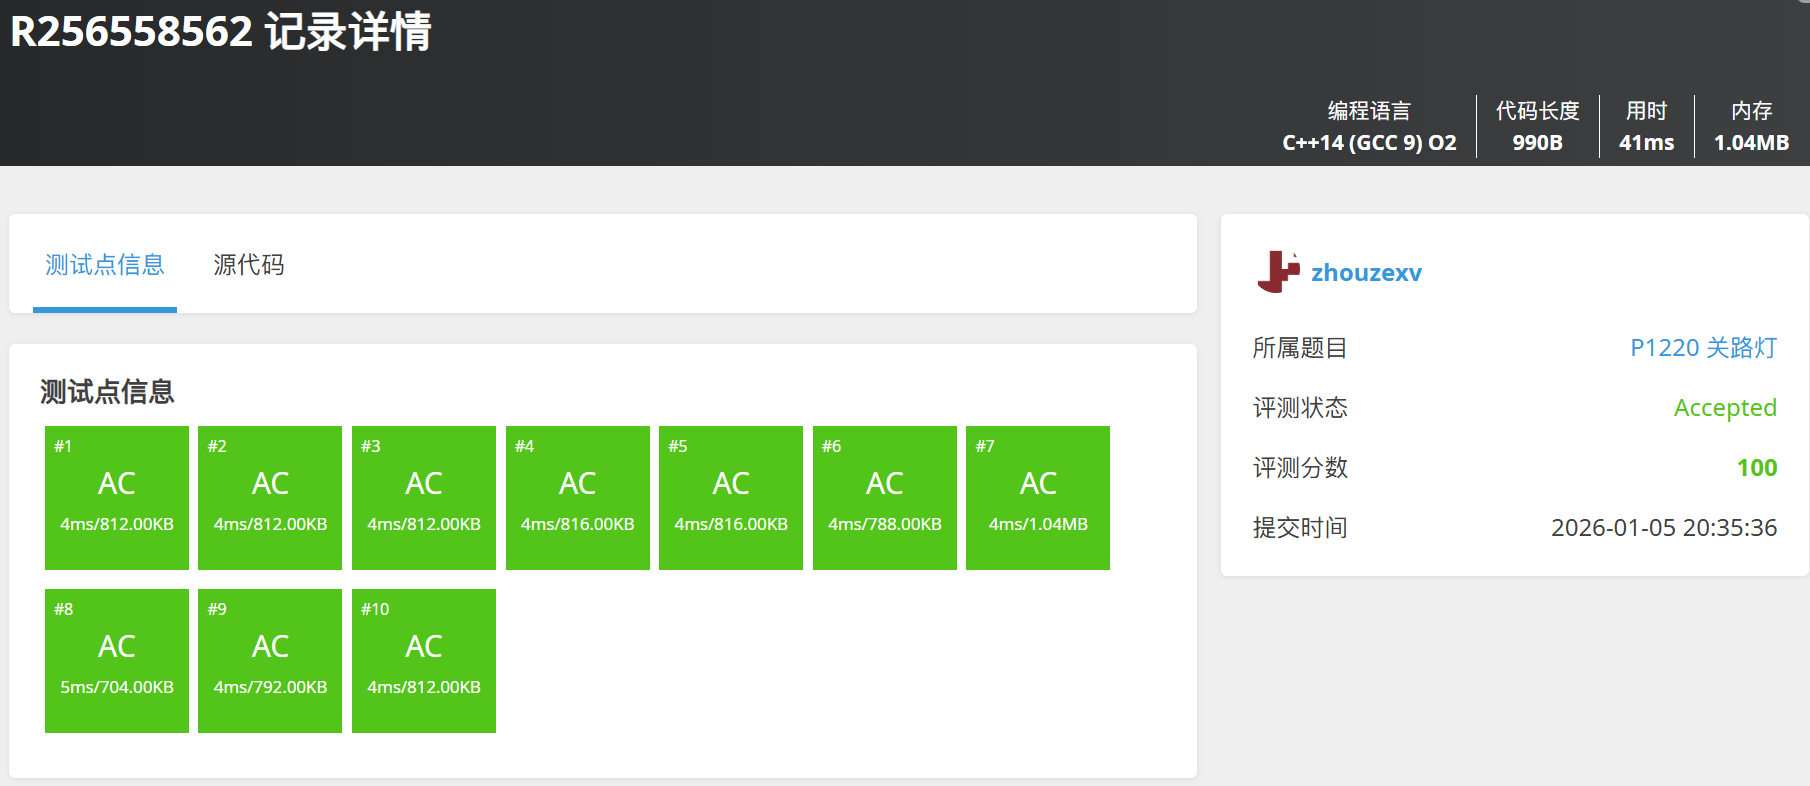
\includegraphics[scale=0.20]{image/P1220.png}
		\caption{P1220运行结果}
		\label{fig5-1}
	\end{center}
\end{figure}

\newpage

\section{P2512糖果传递 解题报告}

\subsection{题目分析}
有 n 个小朋友坐成一圈，每人有 ai个糖果。每人只能给左右两人传递糖果。每人每次传递一个糖果代价为 1。求使所有人获得均等糖果的最小代价。

很显然，如果需要使代价尽可能大，我们可以让两个小朋友把手中的糖果来回反复传递。但这种情况在本题中是需要避免的。例如，1号小朋友需要给2号小朋友一颗糖，就应该直接给2号小朋友一颗糖，而不是先给2号小朋友两颗糖然后2号再退回一颗糖给1号。由此我们可以让糖只在小朋友围成的圈里面单向传递（只顺时针或者只逆时针）。当然这里的单向传递是广义上的单向，如果有必要，传递的糖果数量可以为负数。

虽然提到了传递糖果数可能是负数，直接进行传递也可能导致小朋友手中的糖果数出现负数，但我们不必计较传递的具体方式是否可以实现（但我最初解题的时候总是纠结于具体的传递方式，这显然非常复杂），因为这可以通过小朋友间传递糖果的先后顺序和数量来调整。a先给b糖果x颗b再给c糖果y颗，和b先给c糖果y颗a再给b糖果x颗本质上没有区别。换言之，我们认为小朋友的糖果可以“贷款”，使运算过程中的糖果数为负数。

\subsection{算法设计}
设x[i]为i号小朋友需要给(i+1)号小朋友的糖果数量，每个小朋友最终糖果数即平均糖果数可以表示为$ave = x_{i-1} - x_i + a_i$
于是我们可以得到方程组

对x[i]进行整理，最终得出x[i](i>=2)的通项公式$x_i = x_1 + \sum (a_{i-1} - (i-1) \cdot ave)$，而此题的答案即为所有x的绝对值的和。可以发现后半部分可以用前缀和进行计算，设其为$b_i$，于是可以得到如下设计：
\begin{lstlisting}
b[0]=0;
for(ll i=1;i<n;i++)  b[i]=b[i-1]+ave-a[i];//前缀和
\end{lstlisting}
此处把ave也算入前缀和中方便后续处理。得到最终答案的表达式为：$|x_1 - b_0| + |x_1 - b_1| + \dots + |x_1 - b_{n-1}|$
b[i]可以由题目给出的数据计算得出，由上述通项公式可以看出最终答案只与x[1]有关，即求出这个函数的最小值为最终答案。

有关函数最小值的求解，我们可以抽象为一个数学问题，即数轴上一动点到n个定点的距离之和最小为多少（有点多此一举，不过算是合理联想）。此处先给出结论：选取顶点集中处于中间位置的点，即取x[1]为排序后b[i]数组的中位数即为函数最小值取值处，本题的标签“贪心”二字也终于在此处有所体现。下给出数学证明：
\[
f(x) = \sum_{i=1}^n |x - x_i|
\]我们的目标是找到 x 的取值，使得 f(x) 最小。
下面分情况求解最小值
情况 1：n 为奇数（n=2k+1,k≥0）
当动点 x 取中位数 $x_{k+1}$（即排序后第 k+1 个点的坐标）时，距离之和 f(x) 取得最小值。
最小值计算公式为：
\[
f_{\text{min}} = \sum_{i=1}^{2k+1} |x_{k+1} - x_i|
\]
情况 2：n 为偶数（n=2k,k≥1）
当动点 x 取 中间两个点之间的任意值（即区间 [xk​,xk+1​] 内的任意坐标）时，距离之和 f(x) 取得最小值。
最小值计算公式为：
\[
f_{\text{min}} = \sum_{i=1}^k (x_{2k - i + 1} - x_i)
\]（本质是将两端点配对求和，区间内任意点到每一对点的距离和为定值）
3. 核心原理：绝对值函数的单调性
绝对值函数 $|x−x_i|$ 的导数性质：
\begin{itemize}
    \item 当 $x < x_i$ 时，导数为 $-1$；
    \item 当 $x > x_i$ 时，导数为 $1$；
    \item 当 $x = x_i$ 时，导数不存在（左导数 $-1$，右导数 $1$）。
\end{itemize}

目标函数 $f(x)$ 的导数是各 $|x - x_i|$ 导数的和：
\begin{itemize}
    \item 当 $x$ 在中位数左侧时，导数为负，$f(x)$ 递减；
    \item 当 $x$ 在中位数右侧时，导数为正，$f(x)$ 递增；
    \item 偶数时中间区间导数为 $0$，函数值保持恒定。
\end{itemize}
因此中位数（或中间区间）是函数的极小值点，即最小值点。

于是，我们可以得到如下代码
\begin{lstlisting}
std::sort(b,b+n);
ll x=b[n/2];//取x为b的中位数
\end{lstlisting}
最后我们就可以根据b[i]和x求出最终答案。

\subsection{性能分析}
该题的代码中可以明显看出的复杂度都是$O(n)$级，但其中用到了algorithm库中的sort函数，其时间复杂度一般为$O(n*log n)$，最终整个算法的时间复杂度是$O(n*log n)$。

\subsection{P2512运行测试}

\begin{figure}[htbp!] % here top bottom
	\begin{center}
		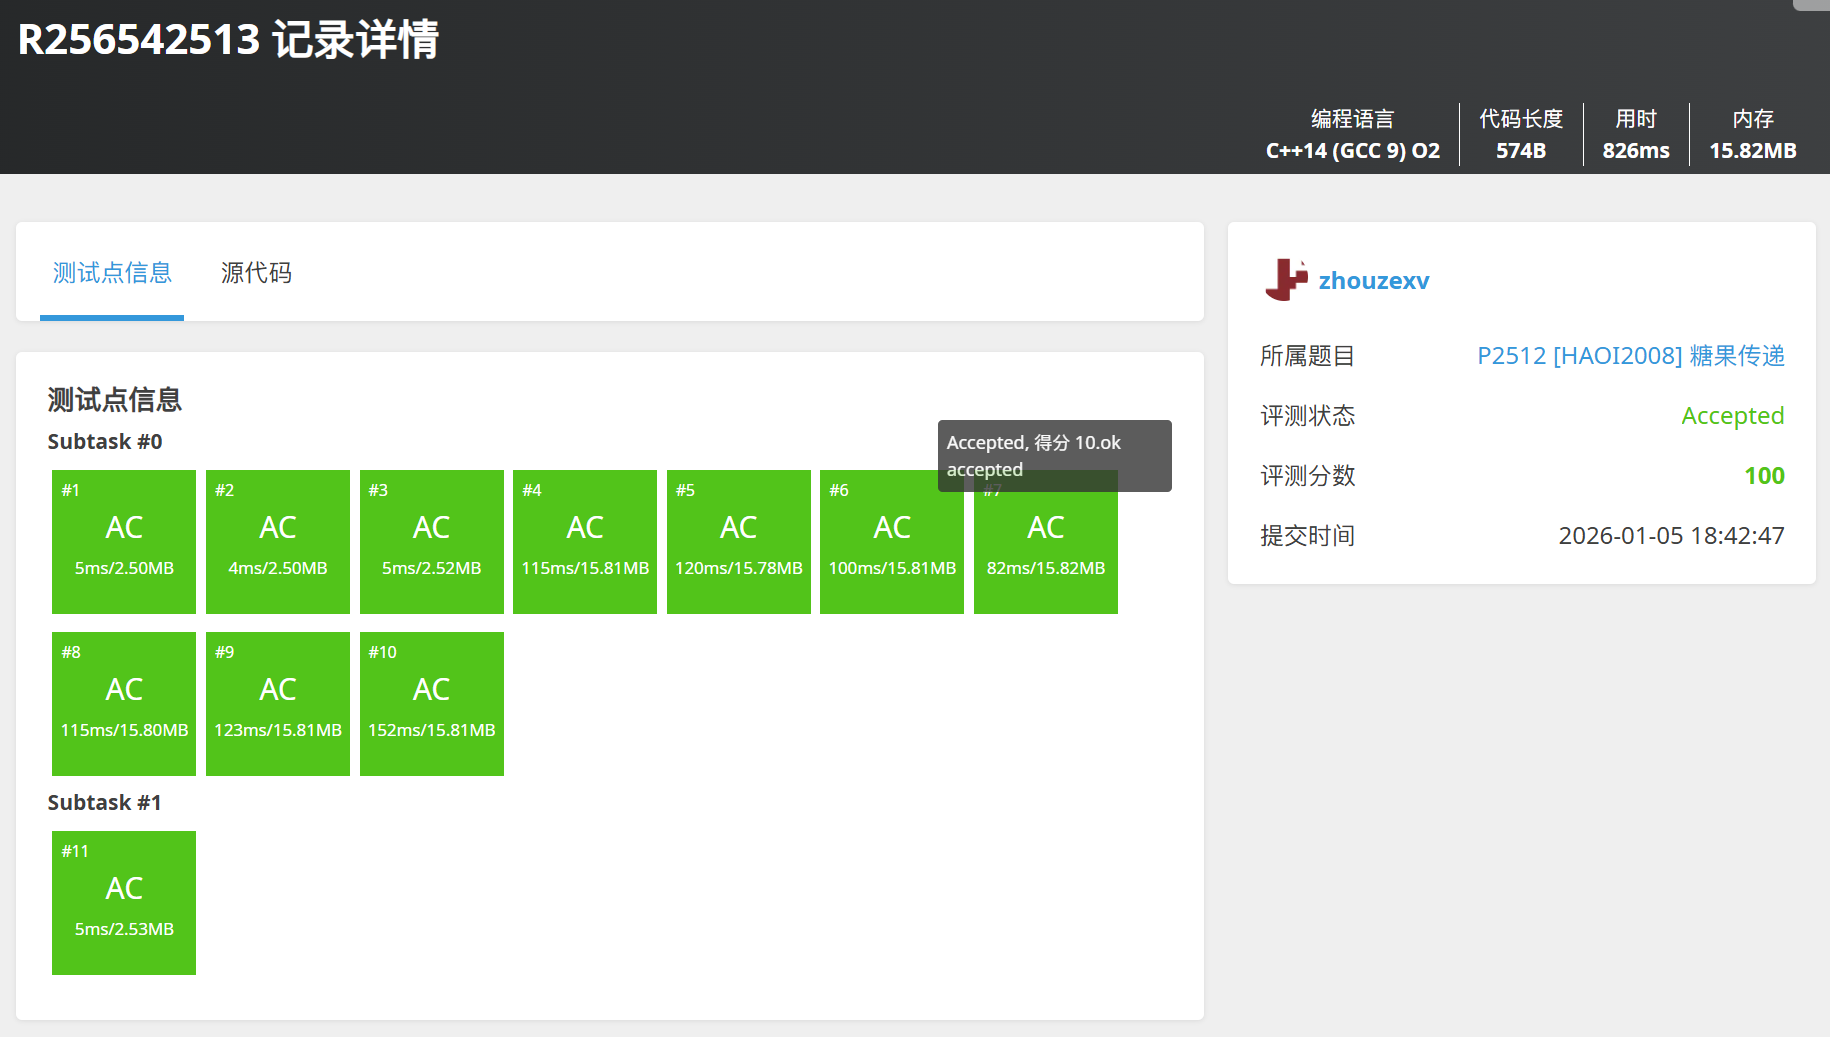
\includegraphics[scale=0.20]{image/P2512截图.png}
		\caption{P2512测试结果}
		\label{fig5-1}
	\end{center}
\end{figure}

\section{P2756  网络流匹配  解题报告}

\subsection{题目分析}
一共有 n 个飞行员，其中有 m 个外籍飞行员和 (n−m) 个英国飞行员，外籍飞行员从 1 到 m 编号，英国飞行员从 m+1 到 n 编号。 对于给定的外籍飞行员与英国飞行员的配合情况，试设计一个算法找出最佳飞行员配对方案，使皇家空军一次能派出最多的飞机。

输入的第一行是用空格隔开的两个正整数，分别代表外籍飞行员的个数 m 和飞行员总数 n。从第二行起到倒数第二行，每行有两个整数 u,v，代表外籍飞行员 u 可以和英国飞行员 v 配合。输入的最后一行保证为 -1 -1，代表输入结束。

请输出能派出最多的飞机数量，并给出一种可行的方案。输出的第一行是一个整数，代表一次能派出的最多飞机数量，设这个整数是 k。第 2 行到第 k+1 行，每行输出两个整数 u,v，代表在你给出的方案中，外籍飞行员 u 和英国飞行员 v 配合。这 k 行的 u 与 v 应该互不相同。

这是一个利用网络流建模最大匹配的模板题，当然也可以用纯粹的匹配算法处理比如匈牙利算法，此处给出网络流建模的题解。

网络流算法有很多种算法，例如FF算法：不断寻找增广路并增加流量，无增广路时的流值即为最大流，具体实现可以使用EK算法，即BFS遍历图寻找增广路，记录每个节点的前驱节点并计算路径上的瓶颈流量，可保证每次寻找的增广路的边数最少，时间复杂度是$O(V*E^2)$。

而本题解将使用Dinic算法，基于FF方法的框架，用分层图和阻塞流进行优化。

接下来我们需要考虑如何将匹配问题建模成网络流图形：可以将外籍飞行员和英国飞行员分别建模为一列点，在有偏好的两个飞行员之间添加一条容量为1的边。然后构造源点s和汇点t，在源点和外籍飞行员之间添加一条容量为1的边，汇点和英国飞行员之间添加一条容量为1的边。这里将边的容量全部设计为1是为了保证每名外籍飞行员只与1名英国飞行员配对。由此可得如下流量图，求出其最大流即为答案。

\begin{figure}[htbp!] % here top bottom
	\begin{center}
		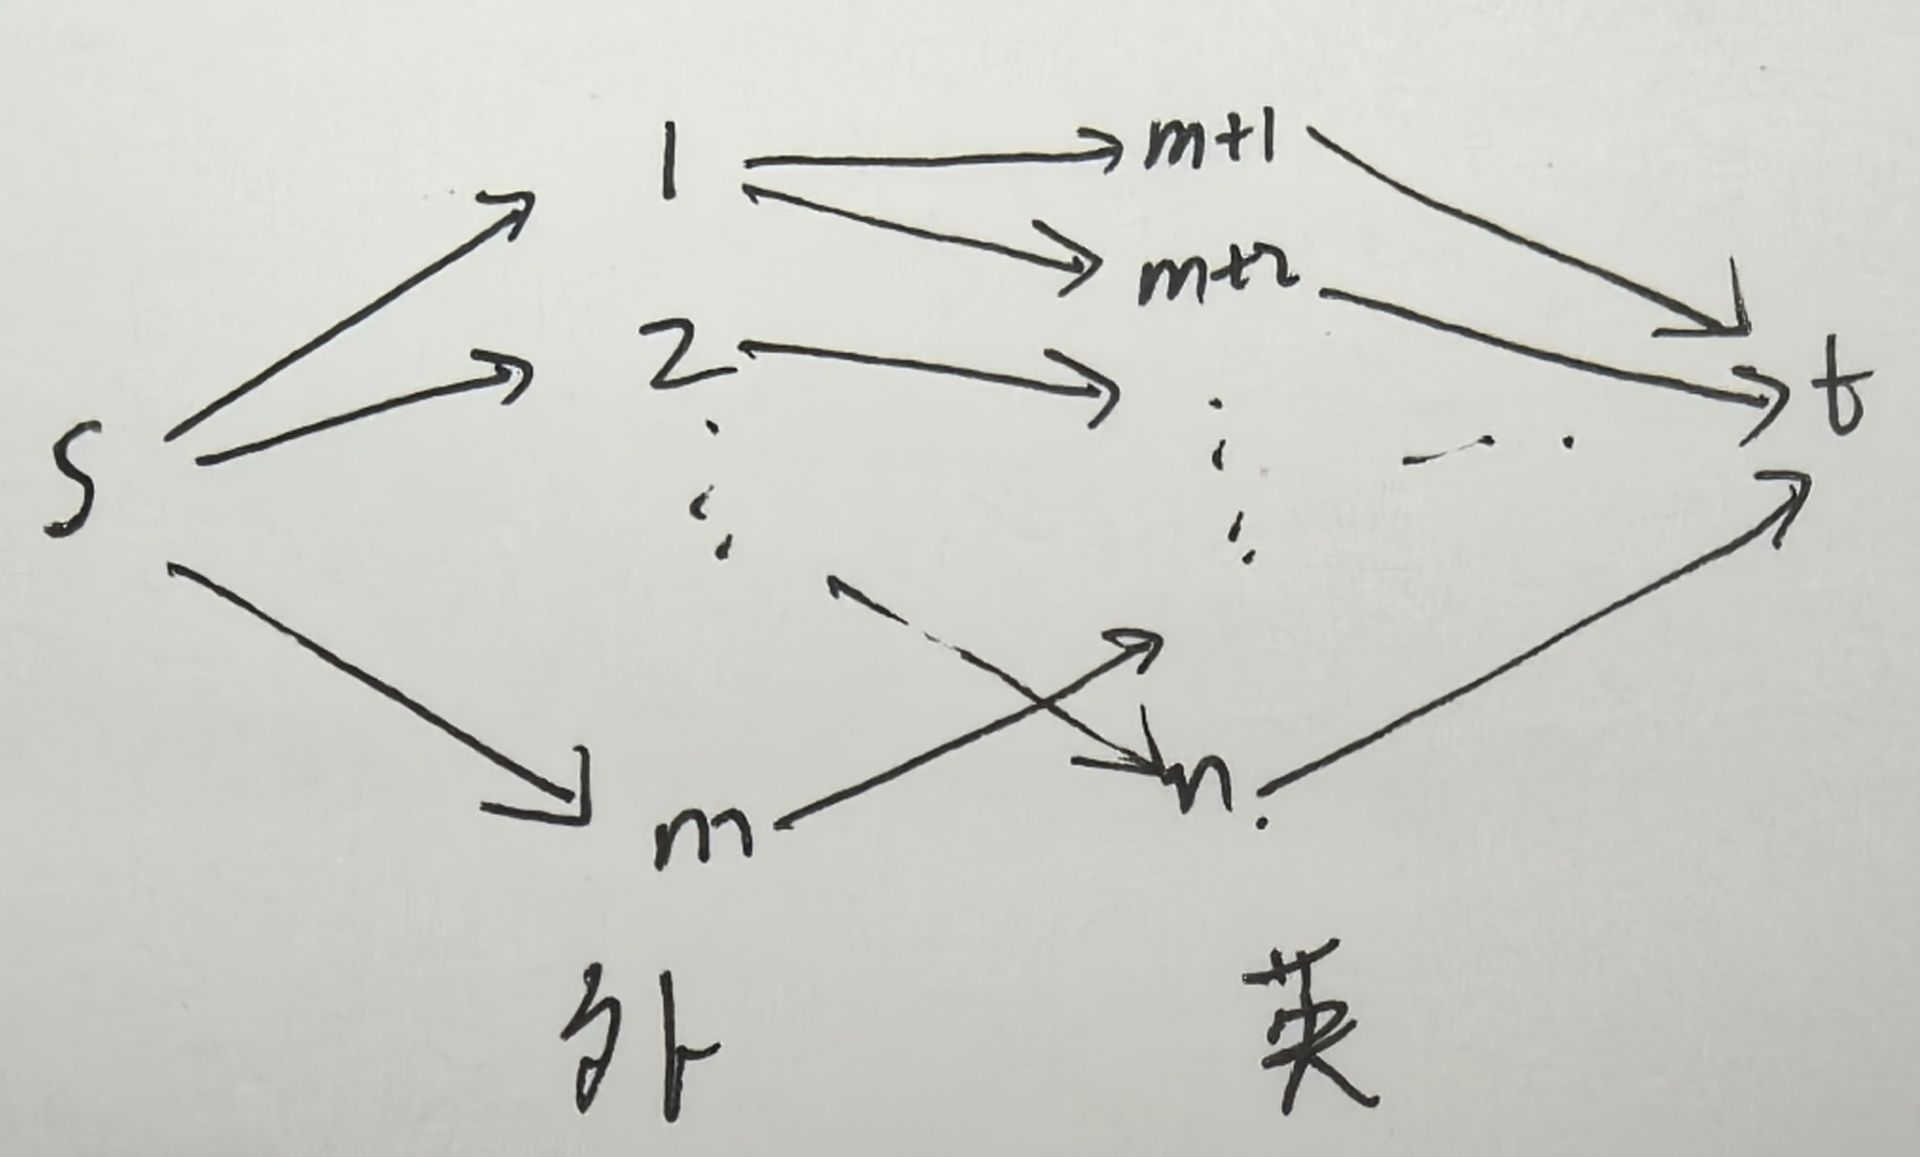
\includegraphics[scale=0.1]{image/网络流建模.jpg}
		\caption{图建模}
		\label{fig5-1}
	\end{center}
\end{figure}

\subsection{算法设计}
首先设计图的数据结构：用结构体封装数据定义边，如下：
\begin{lstlisting}
struct Edge
{
    int to,cap,rev;//to为边的终点,cap为边的容量,rev为反向边的编号
    Edge(int to,int cap,int rev):to(to),cap(cap),rev(rev){}
};
\end{lstlisting}

然后利用构造以Edge为元素的邻接表，edges[u]代表从u出发的所有边，形成图。

level数组用于记录点层数，cur数组用于记录上一次从点出发的边的编号。

在构造有向图的过程中，我们还需要在添加一条边的同时添加这条边对应的反向边。这条反向边的作用是回退流量，其容量是动态的，和正向边实际流量相等，即表示我们最多退回多少流量，使我们有机会修正之前非最优的流量分配。

接下来使用广度优先搜索将图进行分层，用level数组记录，同时可以通过检查汇点是否可达来判断上一步图的构造是否正确。将图进行分层的意义在于后续dfs过程只会从第n层的节点走到第n+1层的节点，禁止同一层中横向行走或者反向行走到第n-1层，避免在图中反复无效搜索。代码如下：
\begin{lstlisting}
bool bfs(int s,int t)//构建分层图
{
    memset(level,-1,sizeof(level));
    queue<int> q;
    level[s]=0;//源点的层数为0
    q.push(s);
    while(!q.empty())
    {
        int u=q.front();
        q.pop();
        for(int i=0;i<edges[u].size();i++)
        {
            Edge &e=edges[u][i];
            if(level[e.to]==-1 && e.cap>0)//如果该点未被访问过且该边有流量
            {
                level[e.to]=level[u]+1;//该点的层数为当前点的层数+1
                q.push(e.to);//将该点入队
            }
        }
    }
    return level[t]!=-1;//如果汇点的层数为-1,则说明汇点不可达,返回false
}
\end{lstlisting}

接下来进行深度优先搜索找出一条流量，同时使用当前弧优化避免遍历所有边，提高效率，cur[u]表示当前遍历到了从u出发的弧的编号，代码实现如下：
\begin{lstlisting}
int dfs(int u, int t, int flow)//从u点出发,到达汇点t,流量为flow
{
    if(u==t) return flow;//如果当前点为汇点,则返回流量
    for(int &i=cur[u];i<edges[u].size();i++)//当前弧优化,从上次出发的边的编号开始遍历
    {
        Edge &e=edges[u][i];
        if(level[e.to]==level[u]+1 && e.cap>0)//如果该点为当前点的下一层且该边有流量
        {
            int min_flow=dfs(e.to,t,min(flow,e.cap));//递归到下一层,流量为当前流量和该边流量的较小值
            if(min_flow>0)//如果下一层有流量
            {
                e.cap-=min_flow;//当前边流量减少
                edges[e.to][e.rev].cap+=min_flow;//反向边流量增加
                return min_flow;//返回流量
            }
        }
    }
    return 0;//如果遍历完所有边都没有流量,则返回0
}
\end{lstlisting}

最后我们将上述DFS和BFS整合到dinic函数中，每次循环先BFS检查汇点是否可达同时构造分层图，若肯定则重置当前弧编号，再反复DFS计算可行路径上的流量直到当前分层图所有路径不再有流量，最后累加得到答案。
\begin{lstlisting}
int dinic(int s, int t)
{
    int max_flow=0;
    while(bfs(s,t))//如果汇点可达
    {
        memset(cur,0,sizeof(cur));//当前弧优化,将所有点的当前弧编号重置为0
        while (int flow=dfs(s,t,INF)) max_flow+=flow;//将源点到汇点的流量加入最大流量
    }
    return max_flow;//返回最大流量
}
\end{lstlisting}

上述代码中对反向边的作用的体现似乎不太直观（其实直到写出这段话的时候我自己还是不太理解），仅在DFS过程中改变流量的时候出现。现在的疑问是，我们已经知道了反向边是为了退回流量设计的，那么它在BFS和DFS是如何发挥作用的，具体是如何操作的？我想办法找了一个例子进行分析：

\begin{figure}[htbp!] % here top bottom
	\begin{center}
		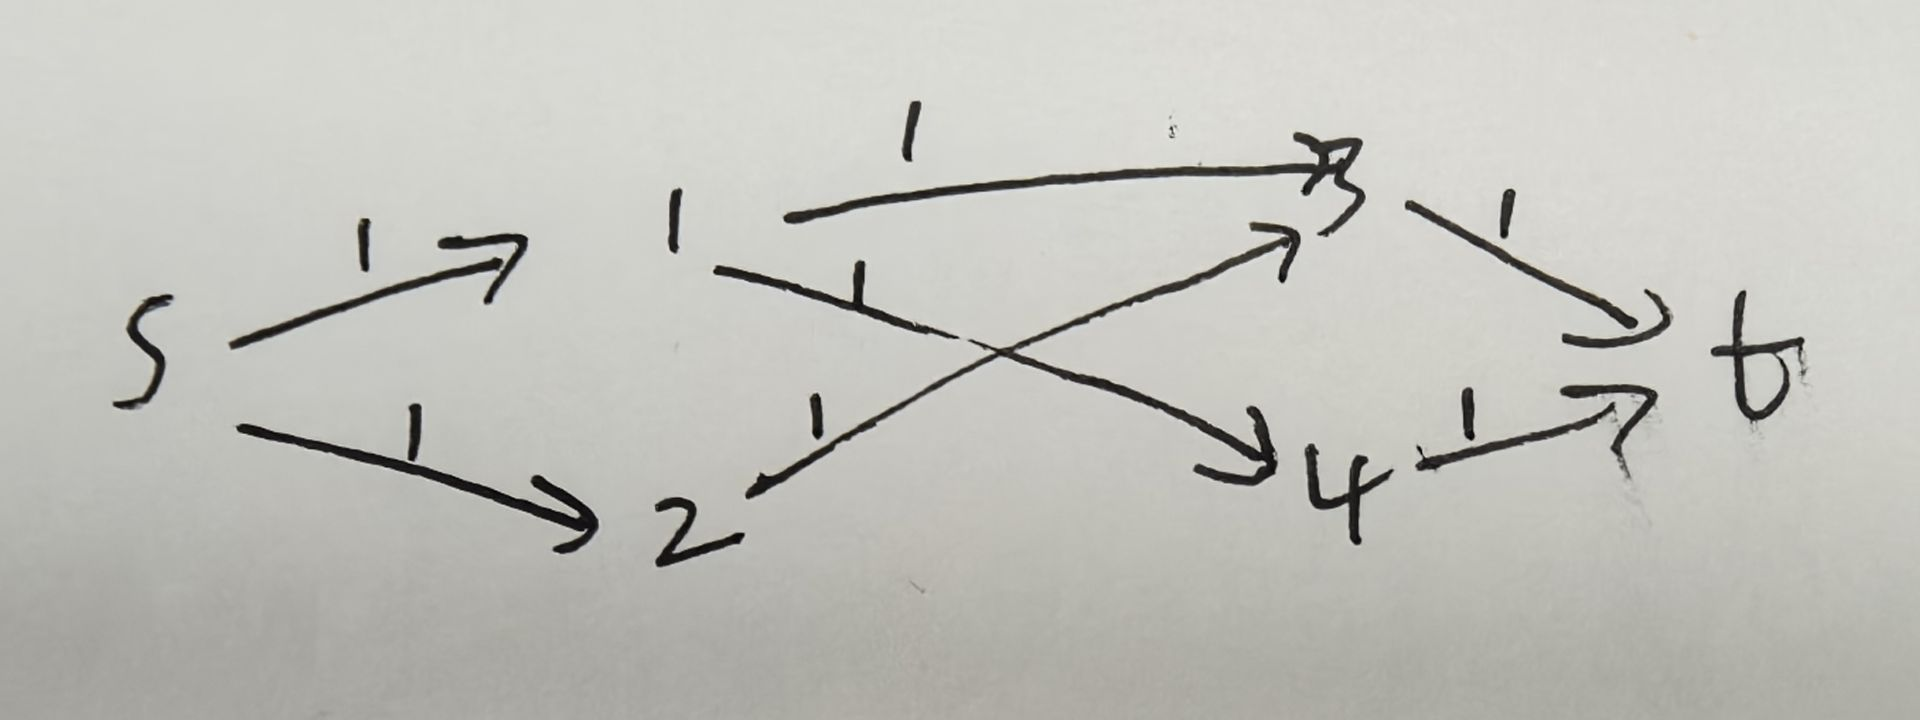
\includegraphics[scale=0.1]{image/网络流示例.jpg}
		\caption{网络流算法示例}
		\label{fig5-1}
	\end{center}
\end{figure}

先BFS分层，再DFS遍历得到s-1-3-t路径，然后s-2-3发现3-t已经没有剩余的容量，此时应该3-1退回1单位流量，原本的s-1-3-t变成s-1-4-t，此时s-2-3-t能够流通。我的理解是把反向边也当做DFS路径的一部分，而不是简单的回退流量寻找更优。这里s-2-3发现堵塞后可以当做DFS的路径继续走3-1-4-t，其中3-1的过程中根据流量处理将1-3流量增加到初始值1，相当于回退流量。由这个思路我们得到的两条路径应该是s-1-3-t和s-2-3-1-4-t，然而总的来看，1-3和3-1相反，相互抵消，然后我们把上述路径中的边重新组合成s-t的路径即为所求s-1-4-t和s-2-3-t。

\subsection{性能分析}

代码的空间消耗主要来自存储图的结构和辅助数组，整体为 $O(E+V)$

Dinic 算法的时间复杂度上限为 $O(V^2 E)$，BFS部分: $O(V + E)$，其中V是节点数，E是边数。DFS部分: $O(V × E)$，在最坏情况下每条边都要遍历一次。

\subsection{P2756运行测试}

\begin{figure}[htbp!] % here top bottom
	\begin{center}
		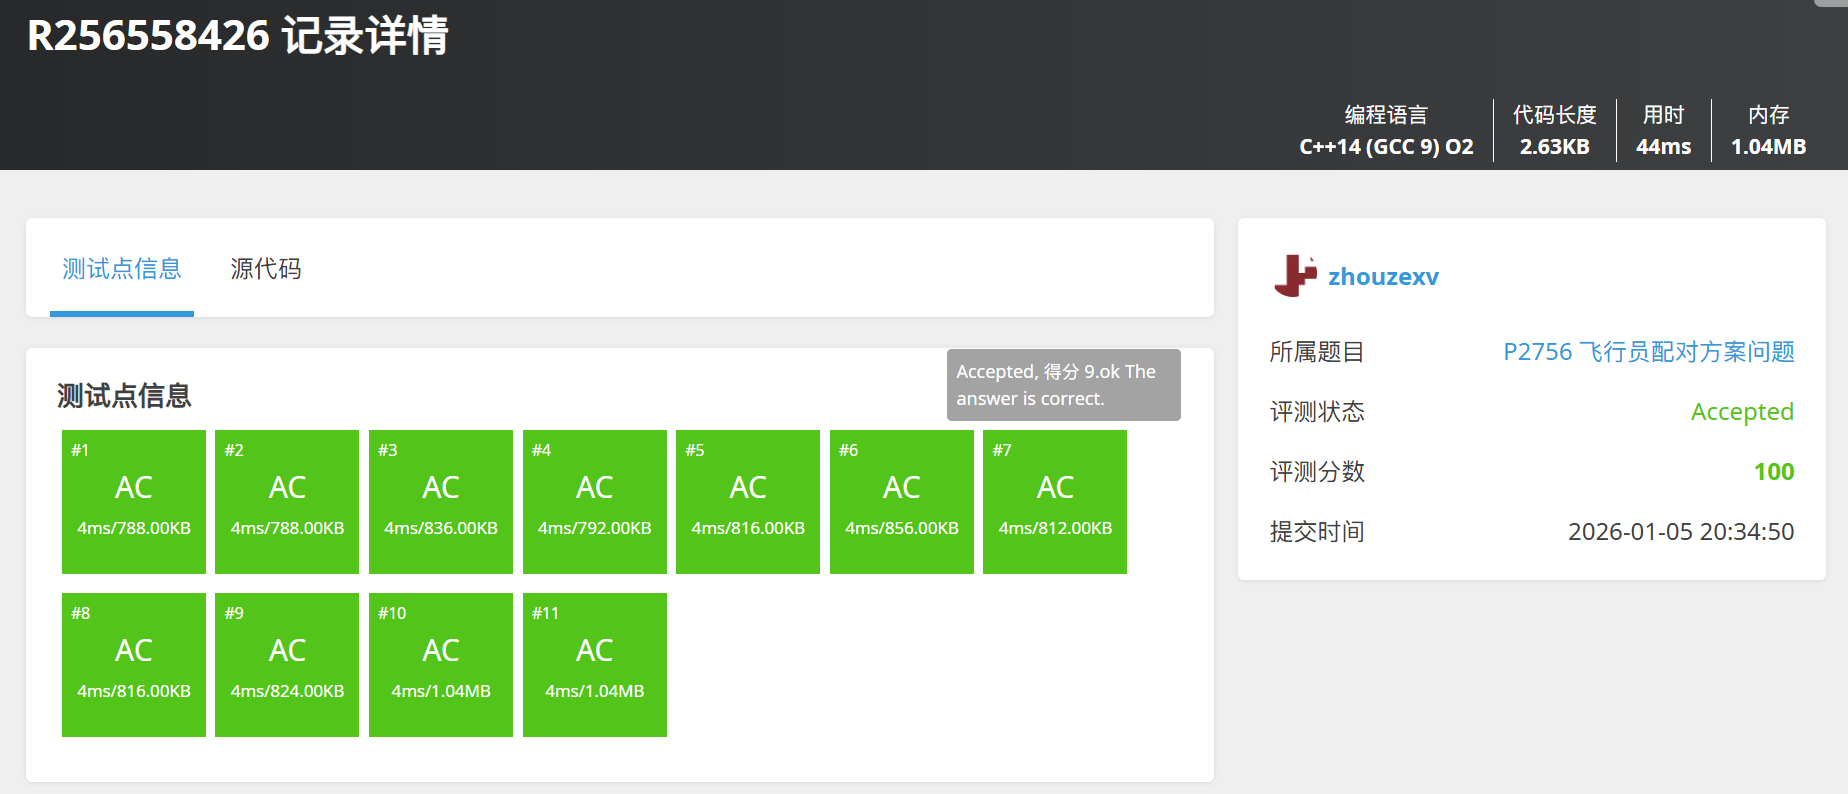
\includegraphics[scale=0.30]{image/P2756.png}
		\caption{P2756测试结果}
		\label{fig5-1}
	\end{center}
\end{figure}

\section{P5691 [NOI2001] 方程的解数  解题报告}

\subsection{题目分析}
给定 n 元高次方程：$a_1 x_1^{k_1} + a_2 x_2^{k_2} + \dots + a_n x_n^{k_n} = 0$，其中约束条件如下：
变量个数 $n \leq 6$，变量取值范围$x_i \in [1,m]$（$m \leq 150$，均为整数）；
每个项的幂次 $k_i \leq 4$，系数 $a_i$ 为整数（可正可负）；要求统计满足方程的整数解的总个数。

一开始我最先想到的就是暴力枚举，毕竟变量取值范围看着不大，但仔细一算就知道完全行不通。当 n=6、m=150 时，总组合数是 1506=1.139×1013，这根本不是计算机能在合理时间内跑完的，暴力枚举直接被 pass。

然后又考虑过贪心算法，能不能优先枚举某些变量来减少计算量？但方程里的系数有正有负，幂次也不一样，根本找不到规律来判断 “先枚举哪个变量更优”，贪心策略只能考虑局部，没法保证全局最优，所以这条路也走不通。

还有动态规划，本来想着能不能通过状态转移来记录中间和，但变量的幂次不统一，系数还能是负数，中间和的范围不好把控，状态定义起来特别复杂，实用性太差。

后来才想到分治的思路，把变量拆成两部分，分别枚举再匹配结果，这样能把指数级的复杂度降下来。而且还要注意一个细节，变量的幂次最高 4 次，系数相乘后可能会是大数，必须用 long long 类型，还不能用 math 库的 pow 函数，不然会有精度误差，我一开始就踩过这个坑，后来换成循环累乘才解决。

对比下来，分治 + 二分查找是最适合这道题的方法，既能保证正确性，又能把复杂度降到可接受的范围。

\subsection{算法设计}

核心思路就是 “拆分变量，分别枚举，匹配结果”。把 n 个变量平均分成左右两部分，比如 n=6 就拆成前 3 个和后 3 个，n=5 拆成前 2 个和后 3 个，这样两部分的枚举规模差不多，优化效果最好。
左部分所有变量的取值组合会算出一堆累加和 sumA，右部分的组合会算出一堆 sumB，方程要满足 sumA+sumB=0，也就是 sumA=−sumB。所以只要把左部分的和存起来排序，再枚举右部分的和，用二分查找找左部分里等于 −sumB 的个数，累加起来就是总解数。

首先我们必须自定义一个幂次计算函数，否则会因为浮点数精度问题导致出错
\begin{lstlisting}
typedef long long ll;
ll powint(int x, int p) {
    ll res = 1;
    for (int i = 1; i <= p; i++) res *= x;
    return res;
}
\end{lstlisting}

接下来是左部分的 DFS 枚举函数，递归遍历所有变量取值，计算累加和并存起来：
\begin{lstlisting}
void dfs_left(int pos, int mid, ll sum) {
    if (pos == mid) { // 枚举完左部分所有变量
        leftsum.push_back(sum);
        return;
    }
    int coeff = a[pos][0];
    int power = a[pos][1];
    for (int i = 1; i <= m; i++) {
        ll temp = coeff * powint(i, power);
        dfs_left(pos + 1, mid, sum + temp);
    }
}
\end{lstlisting}

这里 mid 是拆分点，左部分从 0 到 mid-1，右部分从 mid 到 n-1，这样拆分能保证两部分规模均衡。

然后是右部分的 DFS 枚举，同时用二分查找统计匹配的解数：
\begin{lstlisting}
void dfs_right(int pos, ll sum, int &ans) {
    if (pos == n) { // 枚举完右部分所有变量
        // 找leftsum中等于 -sum 的元素个数
        auto left_it = lower_bound(leftsum.begin(), leftsum.end(), -sum);
        auto right_it = upper_bound(leftsum.begin(), leftsum.end(), -sum);
        ans += right_it - left_it;
        return;
    }
    int coeff = a[pos][0];
    int power = a[pos][1];
    for (int i = 1; i <= m; i++) {
        ll temp = coeff * powint(i, power);
        dfs_right(pos + 1, sum + temp, ans);
    }
}
\end{lstlisting}

plus:经过我的课外研究，发现分治拆分的时候如果不均衡，比如把 n=6 拆成 1 和 5，那时间复杂度就会变成 $O(m^5log m^5)$，效率会差很多，所以一定要平均拆分。

\subsection{性能分析}

时间复杂度方面，左部分枚举的时间是 $O(m^{n/2})$，因为要遍历左部分所有变量的组合；排序 leftsum 的时间是 $O(m^{n/2}*log m^{n/2})$，leftsum 的长度就是 $m^{n/2}$；右部分枚举的时间是 $O(m*{n−n/2})$，每次枚举后二分查找的时间是 $O(log m^{n/2})$。总的来说时间复杂度是 $O(m^{n/2}*log m^{n/2})$。空间复杂度主要来自 leftsum 数组，存储的是左部分所有组合的累加和，空间复杂度是 $O(m^{n/2})$。

还有几个优化点值得一提：一是幂次用循环累乘，避免了 pow 函数的精度误差；二是分治均衡拆分，最大化降低了时间复杂度；三是用二分查找替代哈希表，不用处理哈希冲突，稳定性更高，而且效率也不差。

\subsection{P5691运行测试}
\begin{figure}[htbp!] % here top bottom
	\begin{center}
		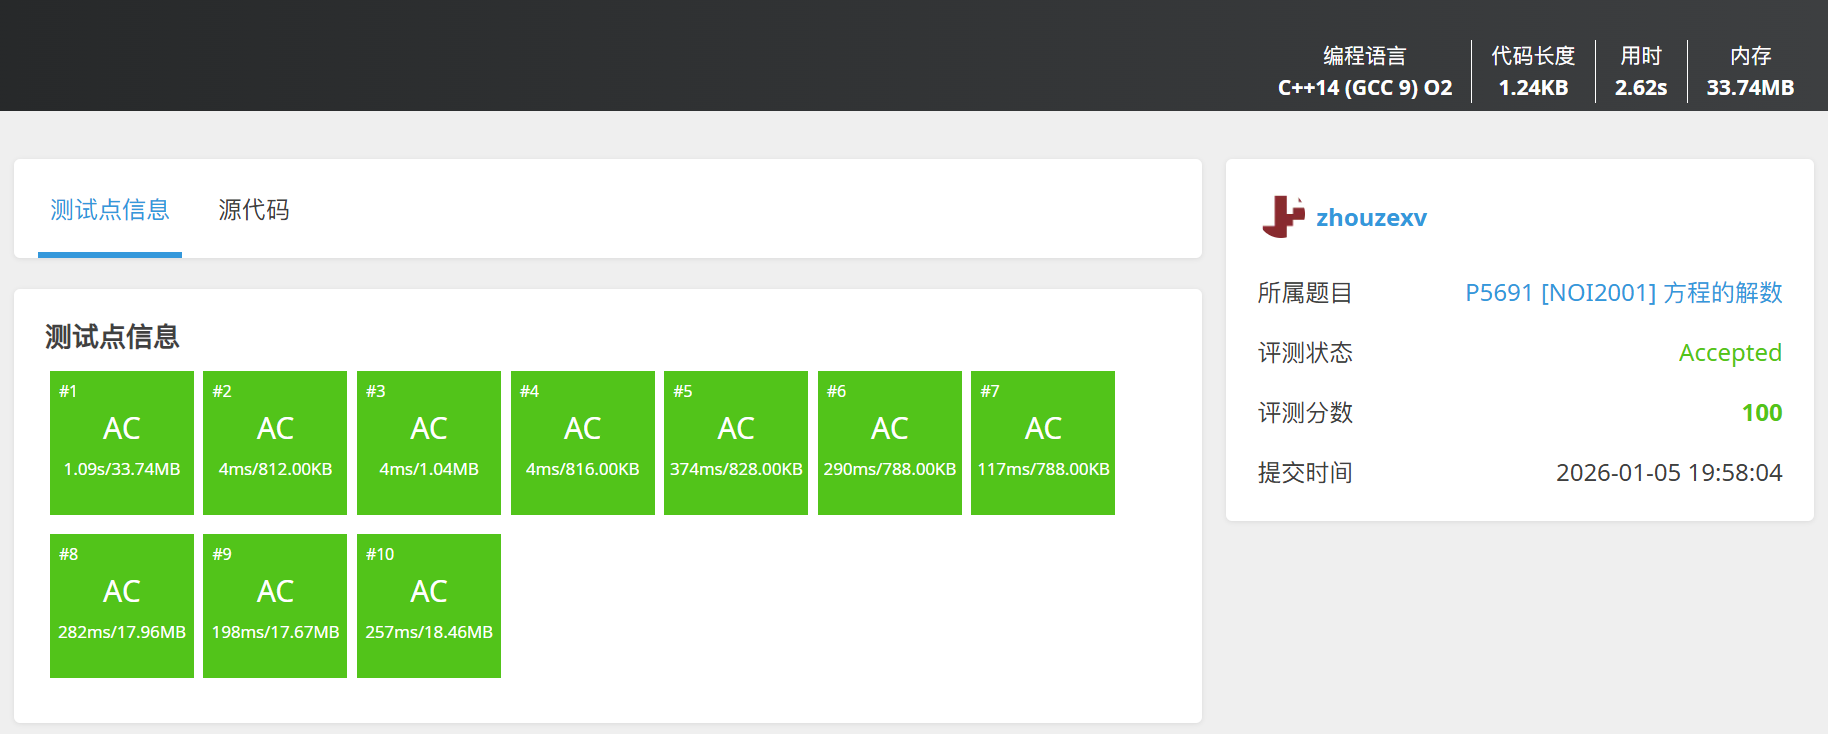
\includegraphics[scale=0.20]{image/P5691截图.png}
		\caption{P5691测试结果}
		\label{fig5-1}
	\end{center}
\end{figure}

\newpage

\section{总结}

\subsection{实验总结}
本次实验中，我通过完成各种题目，巩固了DFS、BFS、Dijstra等经典算法，同时掌握了动态规划、并查集、线段树、分制、贪心等新接触的算法。我的算法设计能力得到提高，写程序也更加得心应手。

通过思考算法的设计与参考其他人的解题思路，我收获了很多经验：

简化代码：本学期我选修了C++程序设计课程，并在课上对C++的stl模板有所了解。相比手动搭建数据结构、手写配套的简单算法函数，使用C++算法模版是一种更高效的选择。例如通过for(auto it:a) 对容器进行遍历，避免了传统 for 循环中冗长的输入，通过sort和自定义的比较函数快速实现排序（可能导致算法超时），还有优先队列、栈等简单数据结构的模版。

问题转换：通过对问题进行建模，我们可以用自己更容易理解的方式看待题目从而快速解决问题。例如飞行员匹配问题，可以建模成网络流问题，当然也可以直接使用对应的匹配算法解决。还有糖果传递问题，将其转换成数学问题之后就能将大部分的运算在草稿纸上实现，剩下来的代码实现过程相对简单。同时，也存在一题多解的情况，如关灯问题中DFS搜索剪枝和动态规划都能解决。

\subsection{个人心得}

我在做题的过程中感触颇深，主要有如下几点思考

做题应该重视原理，不要盲目套模板：模板虽好，题目多变。看到可以套模板的题目很容易导致我们放下警惕而忽略题目中的重要信息。例如有搜索题目看似DFS模板，实则要考虑步数问题。更有汉诺塔问题打着分治递归的旗号，实则思路类似DFS，然而使用类DFS思路解题却只发现可行解，而非最优，这时又可以考虑换成类BFS思路（虽然不方便记录移动过程），或者对类DFS思路进行优化。可见具体问题具体分析，同时要弄清楚算法的基本原理才能解决问题。

空间换时间：最初遇到这个词还是在刚学习哈希表的时候，当时对哈希表的理解还不够深刻，也不懂如何在此之外应用这个思想。现在了解并查集、分治等可以明显降低时间复杂度的算法之后越来越意识到时间的重要性。现在电脑的存储空间越来越大，而人们也越来越要求效率至上，因此适当的空间换取时间是值得提倡的做法。然而这个思维往往与人的正常思维背道而驰，因为我们人脑考虑问题的时候一般找到可行解就够了，我们的解决问题更多在意的是能否解决，至于时间消耗更多和我们的思维灵敏度相关而不是解题方法。但电脑不一样，为电脑设计可行解之后其解题速度远超人脑，此时我们才把目光放在解题方法的优化上。

不足与反思：我对新算法的理解比较滞后，看完讲解之后总是以为自己已经理解，但实际些代码的过程中就发现有些方面不能理解其中的原理，如网络流算法中的反向边的意义。其次缺乏算法优化思维，如关灯问题中想到了可以使用DFS算法，但对于如何剪枝优化时间复杂度没有好的思路。

\subsection{建议}

在第一次写某些算法的过程中我们很可能因为缺乏前置知识导致整个代码无法继续写下去，建议提供一系列从易到难的题目，或者从模板到应用的题单。这样循序渐进更有利于我们自主思考算法的思路，而不是因为在某个缺乏的前置知识上卡住不得不去看题解或者搜索。

实验完成后可以将班级或者年级的优秀代码和解题报告进行汇报展示，供学生交流学习。虽然洛谷也有题解，但有些老题的题解过于久远，偏竞赛风格，往往缺少必要的注释和解析，可读性不高，虽然不同题解之间有互相补充，但还是不便于我们学习，对于算法初学者来说很难理解透彻。

\nocite{*} %% 作用是不对文献进行引用，但可以生成文献列表

\bibliographystyle{Experimental_Report}
\bibliography{Experimental_Report}
\setcounter{secnumdepth}{0}
\appendix

\end{document}